\documentclass[lettersize,journal]{IEEEtran}
\usepackage{amsmath,amsfonts}
\usepackage{algorithmic}
\usepackage{algorithm}
\usepackage{array}
\usepackage[caption=false,font=normalsize,labelfont=sf,textfont=sf]{subfig}
\usepackage{textcomp}
\usepackage{stfloats}
\usepackage{url}
\usepackage{verbatim}
\usepackage{graphicx}
\usepackage{cite}
\usepackage{booktabs}
\usepackage{hyperref}
\usepackage{multirow}
\hyphenation{op-tical net-works semi-conduc-tor IEEE-Xplore}
% updated with editorial comments 8/9/2021

\begin{document}

\title{Learning Annotation-Driven Latent Structure for Multi-Modal Fusion}

\author{
Meilun Zhou,~\IEEEmembership{Graduate Student Member, IEEE},
Aditya Dutt~\IEEEmembership{Member, IEEE},
Alina Zare,~\IEEEmembership{Senior Member, IEEE}%
\thanks{
Meilun Zhou, Aditya Dutt, and Alina Zare are with the Department of Electrical and Computer Engineering, University of Florida, Gainesville, FL, USA.
}%
\thanks{
Alina Zare is also with the Artificial Intelligence and Informatics Research Institute, University of Florida, Gainesville, FL, USA.
}%
}



%         % <-this % stops a space
% \thanks{This paper was produced by the IEEE Publication Technology Group. They are in Piscataway, NJ.}% <-this % stops a space
% \thanks{Manuscript received April 19, 2021; revised August 16, 2021.}}

% % The paper headers
% \markboth{Journal of \LaTeX\ Class Files,~Vol.~14, No.~8, August~2021}%
% {Shell \MakeLowercase{\textit{et al.}}: A Sample Article Using IEEEtran.cls for IEEE Journals}

% \IEEEpubid{0000--0000/00\$00.00~\copyright~2021 IEEE}
% Remember, if you use this you must call \IEEEpubidadjcol in the second
% column for its text to clear the IEEEpubid mark.

\maketitle

\begin{abstract}
Learning shared representations from heterogeneous sensing modalities requires explicitly aligning information that differs in scale, structure, and semantics. Most multi-modal fusion methods rely on downstream task optimization to create cross-modal structure. This work introduces Multi-Modal Continuous Triplet Loss (MMCTL), a representation learning framework that constructs a shared latent space by enforcing similarity relationships derived directly from task annotations. Each modality is processed by a dedicated encoder that maps modality-specific inputs into a common embedding space. MMCTL then applies a continuous triplet loss that compares pairs of samples using annotation-defined similarity, where similarity scores are computed from a weighted combination of classification labels and continuous attributes such as bounding box geometry and object height. Experiments on the AWIR and NEON remote sensing datasets show that this multi-modal alignment yields more coherent and consistently structured latent geometry than unimodal or task-driven fusion approaches.
\end{abstract}

\begin{IEEEkeywords}
Multi-modal representation learning, metric learning, cross-modal alignment, remote sensing.
\end{IEEEkeywords}

\section{Introduction}
\IEEEPARstart{M}{ulti-modal} remote sensing relies on fused representations to integrate complementary sensing modalities \cite{chen2024novel}. Most fusion approaches are developed under a task-driven objective, where fusion is optimized to minimize downstream prediction losses such as classification or regression \cite{bai2025task}. This paradigm can yield strong task accuracy, but it shapes the embedding space only indirectly: distances among samples are not constrained to reflect annotation-defined similarity, so latent geometry becomes a byproduct of whichever prediction objectives are minimized rather than an explicit model of how annotated objects relate.

This gap is especially consequential when supervision mixes categorical labels with continuous attributes. Remote sensing annotations frequently encode size, height, or spatial extent alongside semantic class \cite{sun2023single}. Binary contrastive and classical triplet formulations treat pairs as simply similar or dissimilar \cite{khosla2020supervised}, which discards graded relationships among continuously annotated samples and can flatten intra-class geometric variation. Task-driven fusion likewise encourages decision boundaries that are sufficient for prediction, but does not require that embedding distances remain ordered by continuous annotation proximity across modalities. As a result, fused representations may score well on trained heads while failing to expose an interpretable, annotation-aligned geometry for retrieval, transfer, or multi-attribute reasoning \cite{saidi2024deep}.

This work introduces Multi-Modal Continuous Triplet Loss (MMCTL), which treats multi-modal representation learning as constructing a shared latent space whose geometry is driven by a joint annotation vector. Building on shared-manifold multi-sensor triplets \cite{dutt2022shared} and continuous multi-annotation metric learning \cite{zhou2025multi,kim2019deep}, MMCTL organizes heterogeneous modality embeddings so that relative distances track continuous annotation similarity rather than binary match status or task-loss residuals. Critically, MMCTL uses the \emph{same} annotation sources available to task-driven baselines; the distinction is inductive bias---geometry matching in a shared multi-modal space versus optimizing prediction losses alone. As shown in Fig.~\ref{fig:emb_awir}, paired RGB and thermal embeddings of the same objects occupy nearby regions while class identity and continuous geometric attributes remain structured, in contrast to fusion methods where cross-modal alignment emerges only indirectly from downstream objectives.

% \section{Introduction}
% \IEEEPARstart{M}{ulti-modal} remote sensing typically relies on shared embeddings to integrate different sensing modalities. Most existing fusion approaches focus on improving downstream task performance through architectural coupling or task-specific supervision \cite{houdre2025promm}. While these strategies achieve high task accuracy, they do not explicitly control the geometric structure of the learned embedding space. As a result, representations may collapse nuanced semantic relationships when supervision is heterogeneous or continuous \cite{liu2020global}. Additionally, supervised models are often task-specific, which may limit their generalization across different geographic or temporal domains \cite{houdre2025promm}.

% Most embedding-level fusion methods rely on contrastive formulations that treat all mismatched samples as equally dissimilar. This binary assumption that classifies pairs as either "similar" or "dissimilar" is poorly suited for remote sensing annotations that include continuous attributes such as elevation, moisture content, or biophysical variables. In contrastive frameworks, the reliance on binary pairs can be problematic in remote sensing because diverse images may belong to the same semantic class and lead to encoder collapse or non-informative constant embeddings \cite{choudhury2025rejepa}. This often results in a collapsed embedding space where intra-class variations are ignored, and inter-class distances fail to reflect physical reality \cite{liu2020global}. Furthermore, as supervision sources increase, conflicting task gradients or negative transfer, can distort the shared embedding geometry by forcing shared parameters to optimize for opposing directions \cite{xie2023co, liu2021conflict}. 

% We propose a Continuous Triplet Loss to preserve annotation-grounded geometry rather than enforcing binary similarity. By aligning relative distances in the embedding space with continuous similarity measured in annotation space, this formulation has been shown to learn effective representations under continuous supervision \cite{kim2019deep}. This work applies Continuous Triplet Loss in a multi-modal setting to jointly coordinate embeddings from multiple sensing modalities in a shared latent space using annotation-driven geometry rather than task objectives. As illustrated in Fig.~\ref{fig:emb_awir}, MMCTL coordinates RGB and thermal embeddings from the AWIR dataset so that samples corresponding to the same object are aligned across modalities while preserving semantic separation by class and smooth variation with box size. In contrast, simple concatenation produces disjoint modality clusters with limited cross-modal alignment, and DeepSet fusion \cite{reiter2020deep} fails to clearly separate classes or reflect geometric attributes such as box size. 

\begin{figure*}[!htb]
    \centering
    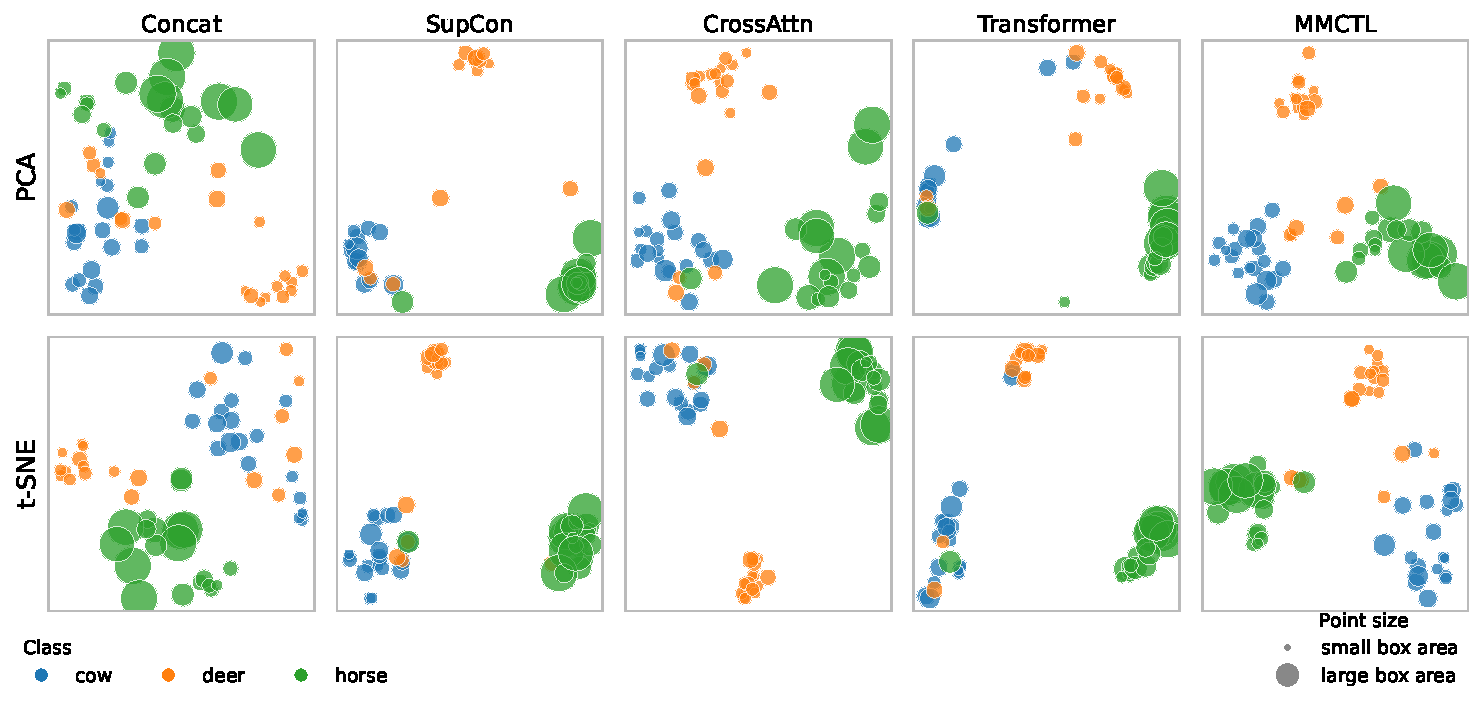
\includegraphics[width=\textwidth]{figures/awir_embedding_space.pdf}
    \caption{AWIR embedding space across fusion methods, projected with PCA (top) and t-SNE (bottom). Points are colored by class label (cow, deer, horse) and sized by bounding-box area. Unimodal (RGB, Thermal) and task-driven fusion (Concat, SupCon, cross-attention, Transformer) embeddings mix classes or show no ordered size gradient, whereas MMCTL yields class-separated clusters in which point size varies smoothly within and across clusters, reflecting the annotation-aligned continuous geometry.}
    \label{fig:emb_awir}
\end{figure*}

\section{Related Work}
\label{sec:related}

Binary supervised contrastive and cross-modal triplets define positives by class or view co-membership with a fixed margin \cite{khosla2020supervised,dutt2022shared}. Continuous metric learning instead couples distances to graded targets \cite{kim2019deep}, including adaptive-margin triplets \cite{ha2021adaptive}. Shared-manifold multi-sensor triplets align heterogeneous modalities for fusion with missing data \cite{dutt2022shared}; our prior multi-annotation continuous triplet organizes a \emph{unimodal} detector from joint class and box labels \cite{zhou2025multi}.

MMCTL contributes: (i)~a joint annotation vector with normalization and task weights (Eqs.~\eqref{eq:ann-norm}--\eqref{eq:ann-concat}); (ii)~a margin-free continuous triplet with adaptive gap $D(\mathbf{y}_a,\mathbf{y}_q)-D(\mathbf{y}_a,\mathbf{y}_p)$ (Eq.~\eqref{eq:mm-adaptive}); (iii)~pairwise distance alignment (Eq.~\eqref{eq:mm-reg}); (iv)~a multi-modal shared space where same-object, different-modality pairs have zero annotation distance. Relative to \cite{zhou2025multi}, MMCTL targets fusion geometry; relative to SupCon or fixed-margin triplets, it replaces hard partitions with annotation-ordered continuous constraints.

\section{Methodology}
\label{sec:methodology}

\subsection{Problem Setup}
\label{subsec:problem-setup}

Consider a multi-modal dataset with $M$ sensing modalities and $N$ instances.
Let $\mathbf{x}_n^{(m)} \in \mathbb{R}^{d_m}$ denote the input for instance
$n \in \{1,\dots,N\}$ from modality $m \in \{1,\dots,M\}$, where $d_m$
denotes the modality-specific input dimensionality.

Each instance is associated with $T$ annotation sources.
For task $t \in \{1,\dots,T\}$, the annotation for instance $n$ is represented
by a row vector
\[
\mathbf{y}^{t}_{n}
=
\big[
y^{t}_{n,1}\;\; y^{t}_{n,2}\;\; \dots\;\; y^{t}_{n,L_t}
\big]
\in \mathbb{R}^{1 \times L_t},
\]
where $L_t$ denotes the number of annotation features for task $t$.

To ensure comparability across annotation sources with different scales,
each annotation feature is normalized independently to the interval $[0,1]$
using statistics computed from the training set only.
Let $\mathcal{N}_{\mathrm{train}} \subset \{1,\dots,N\}$ denote the index set of
training instances.

For each task $t$ and annotation feature index $\ell \in \{1,\dots,L_t\}$, define the
training-set extrema
\[
\mu^{t}_{\min,\ell}
=
\min_{n \in \mathcal{N}_{\mathrm{train}}} y^{t}_{n,\ell},
\qquad
\mu^{t}_{\max,\ell}
=
\max_{n \in \mathcal{N}_{\mathrm{train}}} y^{t}_{n,\ell}.
\]

\noindent Normalization is applied feature-wise as
\begin{equation}
\label{eq:ann-norm}
\tilde{y}^{t}_{n,\ell}
=
\frac{
y^{t}_{n,\ell}
-
\mu^{t}_{\min,\ell}
}{
\mu^{t}_{\max,\ell}
-
\mu^{t}_{\min,\ell}
},
\qquad
\forall \ell \in \{1,\dots,L_t\}.
\end{equation}

\noindent The same normalization parameters are reused unchanged for validation and test instances. After normalization, annotation vectors are rescaled to account for differences in dimensionality across tasks.
Let
\[
L_{\max} = \max_{t \in \{1,\dots,T\}} L_t .
\]
Each normalized annotation vector is scaled and weighted as
\begin{equation}
\label{eq:ann-weight}
\hat{\mathbf{y}}^{t}_{n}
=
w_t \, \tilde{\mathbf{y}}^{t}_{n}\, \frac{L_{\max}}{L_t},
\end{equation}
where $w_t \ge 0$ is a fixed hyperparameter controlling the influence of task $t$. Feature-wise min--max normalization and the $L_{\max}/L_t$ length correction are therefore already encoded in Eqs.~\eqref{eq:ann-norm}--\eqref{eq:ann-weight}; the only free annotation knobs are the task weights $\{w_t\}$. In the main experiments we fix $w_{\text{class}}{=}0.5$ on AWIR and $w_{\text{class}}{=}1.0$ on NEON (with continuous-task weights at $1.0$) to balance semantic and geometric sources.

The final joint annotation vector for instance $n$ is constructed by horizontal
concatenation:
\begin{equation}
\label{eq:ann-concat}
\mathbf{y}_{n}
=
\big[
\hat{\mathbf{y}}^{1}_{n}
\;\;
\hat{\mathbf{y}}^{2}_{n}
\;\;
\dots
\;\;
\hat{\mathbf{y}}^{T}_{n}
\big]
\in
\mathbb{R}^{1 \times L},
\end{equation}
where $L = \sum_{t=1}^{T} L_t$.
This joint annotation vector defines a unified similarity space whose geometry
reflects relationships across all annotation sources.


\subsection{Shared Latent Space with Modality-Specific Encoders}
\label{subsec:shared-latent-space}
Multi-modal observations provide complementary and non-redundant information about each instance, as different sensing modalities capture distinct physical, spectral, or geometric properties. Leveraging these complementary cues requires a representation that preserves modality-specific information while enabling direct comparison and alignment across modalities. To this end, each modality is processed by a dedicated encoder that maps modality-specific inputs into a shared latent space.

Each modality is processed by a dedicated encoder
$e_m(\cdot)$ that maps modality-specific inputs into a shared latent space.
For instance $n$ and modality $m$,
\begin{equation}
\mathbf{z}_n^{m}
=
e_m\!\left(\mathbf{x}_n^{m}\right),
\qquad
\mathbf{z}_n^{m} \in \mathbb{R}^{F},
\end{equation}
where $F$ denotes the shared embedding dimension.

Similarity in both annotation space and latent space is measured using cosine
distance,
\begin{equation}
D(\mathbf{u},\mathbf{v})
=
1 -
\frac{
\mathbf{u}^{\top}\mathbf{v}
}{
\|\mathbf{u}\|_2 \|\mathbf{v}\|_2
}.
\end{equation}

Triplets are formed with a \emph{batch-all} strategy. Within each mini-batch, every index may serve as an anchor $a$. For that anchor, a pair $(p,q)$ is a valid (positive, negative) pair if and only if
\begin{equation}
\label{eq:triplet-order}
D(\mathbf{y}_a,\mathbf{y}_p)
<
D(\mathbf{y}_a,\mathbf{y}_q).
\end{equation}
Positives and negatives are therefore defined solely by annotation-distance ordering: any sample closer to the anchor in joint annotation space than another is treated as relatively more similar. There is \emph{no} hard similarity threshold that partitions pairs into absolute positives and negatives, and no class-equality rule beyond what is already encoded in $\mathbf{y}_n$.

Let $K$ denote the number of valid triplets in a batch under this batch-all construction. The multi-modal continuous triplet loss is
\begin{equation}
\label{eq:mm-adaptive}
\begin{aligned}
\mathcal{L}_{\text{mm\_adaptive}}
=
\sum_{k=1}^{K}
\Big(
& \max\!\big(
D(\mathbf{z}_{a_k},\mathbf{z}_{p_k})^2
-
D(\mathbf{z}_{a_k},\mathbf{z}_{q_k})^2 \\
& \quad +
D(\mathbf{y}_{a_k},\mathbf{y}_{q_k})
-
D(\mathbf{y}_{a_k},\mathbf{y}_{p_k}),
\, 0
\big)
\Big).
\end{aligned}
\end{equation}
There is no fixed margin hyperparameter. The term $D(\mathbf{y}_{a},\mathbf{y}_{q})-D(\mathbf{y}_{a},\mathbf{y}_{p})$ acts as an adaptive, annotation-derived margin: the required embedding separation equals the annotation-distance gap for that triplet.

To encourage consistency between annotation-defined geometry and embedding
geometry, a regularization term enforces pairwise distance alignment,
\begin{equation}
\label{eq:mm-reg}
\begin{aligned}
\mathcal{L}_{\text{mm\_reg}}
=
\sum_{k=1}^{K}
\Big(
& \left(
D(\mathbf{z}_{a_k},\mathbf{z}_{p_k})
-
D(\mathbf{y}_{a_k},\mathbf{y}_{p_k})
\right)^2 \\
& \quad +
\left(
D(\mathbf{z}_{a_k},\mathbf{z}_{q_k})
-
D(\mathbf{y}_{a_k},\mathbf{y}_{q_k})
\right)^2
\Big).
\end{aligned}
\end{equation}
The final Multi-Modal Continuous Triplet Loss is
\begin{equation}
\mathcal{L}_{\text{mm\_ctl}}
=
\mathcal{L}_{\text{mm\_adaptive}}
+
\mathcal{L}_{\text{mm\_reg}}.
\end{equation}

When the same instance is observed across multiple modalities, identical joint
annotation vectors yield zero annotation distance. This property encourages
embeddings of the same physical object from different sensing modalities to
align in the shared latent space while preserving continuous variation across
distinct instances.


\subsection{Modality-Specific Encoder Architecture}

Each sensing modality is first encoded using a dedicated convolutional autoencoder trained independently with a standard reconstruction objective. This design allows each encoder to specialize in extracting features aligned with the physical characteristics and information content of its corresponding modality, without imposing cross-modal constraints during representation learning.

For hyperspectral imagery, the encoder architecture emphasizes spectral feature extraction. The network uses $1 \times 1$ convolutions to model per-pixel spectral relationships, followed by densely connected layers that capture higher-order spectral interactions. Global average pooling is applied at the final convolutional stage to aggregate spectral responses into a fixed-length representation. For RGB, thermal, and LiDAR modalities, the encoder architecture emphasizes spatial structure. These encoders use spatial convolutions organized into dense blocks to capture local and contextual spatial patterns present in each modality. Global average pooling is applied after the final dense block to produce a compact representation that is invariant to spatial resolution.

In all cases, the encoder outputs a $1024$-dimensional latent embedding vector. Modality-specific autoencoders are first pretrained independently with reconstruction objectives. For all fusion methods evaluated here---including concatenation, SupCon, cross-attention, Transformer fusion, and MMCTL---those modality encoders are then frozen, and fusion operates on fixed embeddings. This two-stage freeze is a \emph{fair fusion evaluation protocol}: it isolates shared-space organization from differences in modality-specific feature learning, so that downstream gaps reflect fusion geometry rather than unequal encoder capacity. Under this protocol, MMCTL trains only the shared multi-modal organization with annotation-derived distance supervision (Section~\ref{subsec:shared-latent-space}); after MMCTL training, the resulting embeddings are frozen and lightweight task heads are trained separately, as shown in Fig.~\ref{fig:MMCTL_Training_Architecture}. End-to-end unfreezing of modality encoders is left for optional follow-up comparison and is not required for the protocol used throughout the main tables.

\begin{figure}[!htb]
    \centering
    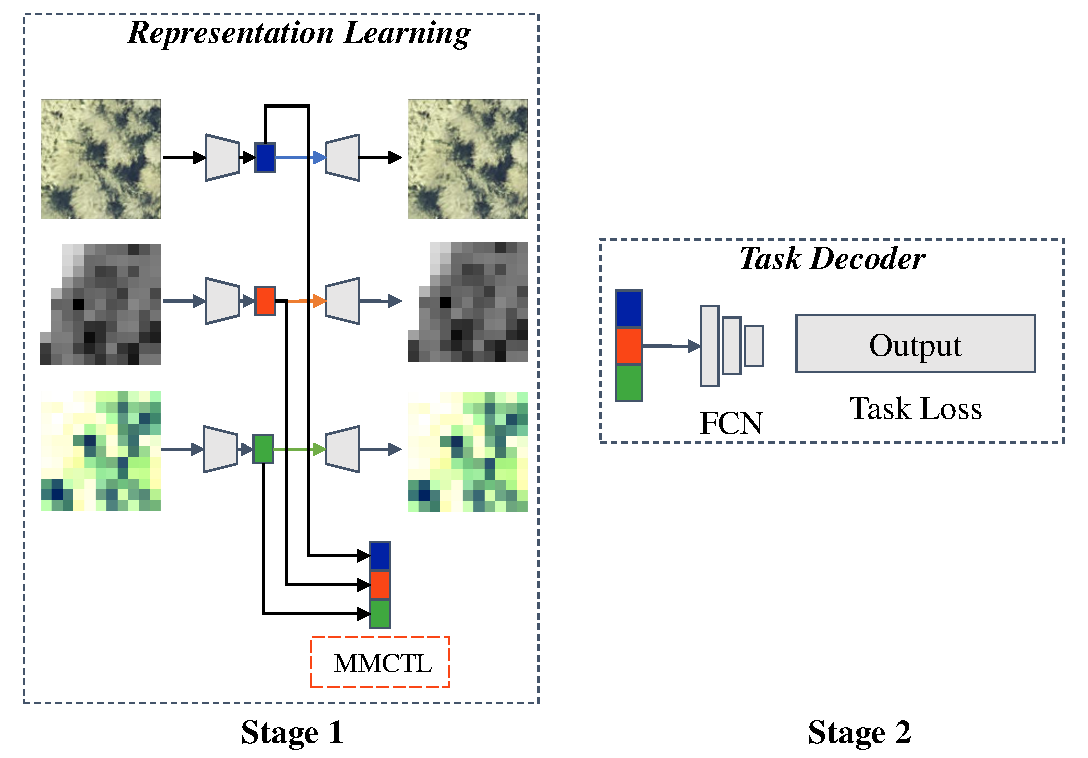
\includegraphics[width=\columnwidth]{figures/MMCTL-Framework-Figure.pdf}
    \caption{Two-stage MMCTL training on NEON under the frozen-encoder fusion protocol. Modality-specific encoders are pretrained and frozen; MMCTL organizes the shared latent space with Continuous Triplet Loss over a joint annotation vector; task-specific heads are then trained independently to assess representation quality.}
    \label{fig:MMCTL_Training_Architecture}
\end{figure}

\section{Experiments}

\subsection{Datasets and Modalities}
\label{subsec:datasets}

Experiments are conducted on two remote sensing datasets that differ in sensing modalities, spatial resolution, and annotation structure. These datasets provide complementary test cases for evaluating multi-modal embedding fusion under heterogeneous sensing conditions.

The first dataset is Animal Wildlife Image Repository (AWIR) \cite{samiappan2024aerial, zhou2025multi}, which contains paired RGB and thermal imagery observing the same objects and spatial regions. RGB provides high-resolution visual appearance, while thermal supplies complementary temperature-based cues. The data processing follows the existing pipeline \cite{zhou2025multi}. The NEON dataset is derived from the NeonTreeEvaluation Benchmark \cite{Weinstein_Marconi_White_2022} and includes aligned RGB, hyperspectral, and LiDAR data from NEON airborne products. Tree crowns are centered on stem locations with species labels from NEON vegetation structure data \cite{NEON_vegetation_structure}. Species labels are provided per stem, crown polygons yield geometric attributes, and height statistics are computed from LiDAR-derived canopy height models, including minimum, maximum, mean, and standard deviation of height. We extract $6\times6$ patches at $1\,\mathrm{m}$ for hyperspectral and CHM and $60\times60$ patches at $10\,\mathrm{cm}$ for RGB, then apply Min-Max normalization using training statistics.

\subsection{Experimental Setup}
Evaluation targets embedding-level fusion under a two-stage frozen-encoder protocol (Section~\ref{sec:methodology}). For all comparison methods, modality-specific encoders are frozen and fusion operates on fixed embeddings. Task-driven fusion methods observe the same annotation sources as MMCTL, but consume them through supervised prediction losses during fusion training; MMCTL instead uses those annotations to define continuous distances for geometry matching (Section~\ref{subsec:shared-latent-space}). The claim is therefore not that MMCTL forgoes labels, but that it applies a different inductive bias to the same label sources. Datasets are split into $50\%$ training and $50\%$ test sets, with the test set excluded from model selection. Within the training split, $k$-fold cross-validation is used for model selection and uncertainty reporting: $8$ folds for AWIR and $5$ folds for NEON. All splits use a fixed random seed, and each reported mean~$\pm$~std is computed across these folds (i.e., the ``runs'' in figure captions are the CV folds). Categorical annotations use a fixed weight of $w_{\text{class}} = 0.5$ in the joint annotation vector for the AWIR dataset and $1.0$ for the NEON dataset to balance with continuous annotations.

Comparisons include concatenation and three stronger fusion baselines requested for this revision: supervised contrastive fusion (SupCon) \cite{khosla2020supervised}, cross-attention pooling, and a small Transformer encoder over modality tokens. Concatenation stacks modality embeddings and remains untrained. SupCon learns a projection of the concatenated embeddings with class-supervised contrastive loss. Cross-attention and Transformer fusion are trained with the same task supervision used previously for DeepSet baselines (classification plus continuous regression). These methods contrast with MMCTL, which organizes latent geometry using annotation-derived similarity rather than prediction losses alone.

Next, task heads are optimized using supervised losses appropriate to each task, with identical architectures and optimization settings across all fusion methods. Training runs for up to $3000$ epochs with early stopping based on validation performance and a patience of $1000$ epochs. Optimization uses Adam with a learning rate of $10^{-3}$ and weight decay of $10^{-4}$. Batch size is set to $4$ for AWIR with no gradient clipping applied, while NEON uses a batch size of $32$ with gradient clipping enabled at a norm of $5$. Task heads use a shallow multilayer perceptron for both classification and regression tasks. Code for reproducing all experiments can be found at
\href{https://github.com/GatorSense/MMCTL}{github.com/GatorSense/MMCTL}.

\paragraph{Reproducibility.}
AWIR and NEON tables use released full-set embeddings ($N{=}240$ AWIR; $N{=}592$ NEON) with independently trained unimodal encoders and MMCTL. SupCon, cross-attention, and Transformer fusion are trained on frozen unimodal embeddings under a $50/50$ holdout plus $k$-fold protocol ($8$ AWIR / $5$ NEON) and paper task-head settings (Adam, $3000$ epochs, patience $1000$).

\subsection{Latent Space Quality Metrics}
\label{sec:latent_space_quality_metrics}
Latent space structure is evaluated using simple global and local metrics that quantify alignment with annotation-defined geometry.

\paragraph{Global Consistency}
Let $\mathbf{z}_i \in \mathbb{R}^{d}$ denote the normalized embedding of sample $i$, and let $y_i^{(s)}$ denote the annotation for supervision source $s \in \{\mathrm{cls}, \mathrm{box}, \mathrm{pos}, \mathrm{height}\}$. For a pair $(i,j)$, embedding distance is $d_E(i,j) = \lVert \mathbf{z}_i - \mathbf{z}_j \rVert_2$, with annotation distance $d_s(i,j)$. Global consistency is
\begin{equation}
A_s
=
\mathbb{E}_{(i,j)}
\left[
\frac{d_E(i,j)}{d_s(i,j) + \epsilon}
\right],
\end{equation}
where lower values indicate stronger geometric alignment.

\paragraph{Local Smoothness}
Let $\mathcal{N}_k(i)$ denote the $k$ nearest neighbors of $\mathbf{z}_i$. Local smoothness is defined as
\begin{equation}
S_s(k)
=
\mathbb{E}_{i}
\left[
\operatorname{std}
\big(
\{ y_j^{(s)} : j \in \mathcal{N}_k(i) \}
\big)
\right],
\end{equation}
where lower values indicate greater annotation consistency among neighbors.

\paragraph{Structure Score}
For compact comparison, metrics are standardized across representations. The structure score is defined as
\begin{equation}
\mathrm{Struct}_s(k)
=
Z^{A}_s
+
Z^{S}_s(k),
\end{equation}
with lower values indicating stronger structure preservation. All experiments use $k=3$.

% Cosine distance is used during MMCTL training, while Euclidean distance is used for evaluation.



\subsection{Experimental Results}
Latent space structure is first evaluated using the global consistency and local smoothness metrics defined in Subsection~\ref{sec:latent_space_quality_metrics}. Table~\ref{tab:latent_alignment} compares structure scores across unimodal encoders, fusion methods, and MMCTL.

Across both datasets, standard fusion methods such as concatenation and task-driven attention can improve over unimodal encoders, but geometric alignment across supervision sources remains uneven. In contrast, MMCTL achieves the strongest class and height structure on NEON and remains competitive with cross-attention on box structure, while on AWIR it produces the best structure across all supervision sources. These results indicate that annotation-driven multi-modal supervision yields more coherent and consistently aligned latent geometry than fusion strategies optimized only for prediction.


\newcommand{\err}[1]{\,\scriptstyle\pm\,\!#1}

\begin{table}[t]
\centering
\caption{
Latent space structure score across datasets. Fusion baselines are concatenation, SupCon, cross-attention, and Transformer pooling (DeepSet omitted). Annotation types include C for class labels, B for box, P for position, and H for height annotations.
}
\label{tab:latent_alignment}
\begin{tabular}{l c c c c}
\toprule
\textbf{Dataset} & \textbf{Method} 
& \textbf{C} $\downarrow$
& \textbf{B} $\downarrow$
& \textbf{P} $\downarrow$ \\
\midrule
\multirow{7}{*}{AWIR}
& RGB           
& $\phantom{-}1.85\err{0.16}$ 
& $-0.77\err{0.11}$ 
& $-0.07\err{0.15}$ \\
& Thermal       
& $\phantom{-}2.02\err{0.22}$ 
& $\phantom{-}1.50\err{0.10}$ 
& $\phantom{-}2.40\err{0.24}$ \\
\cmidrule(lr){2-5}
& Concat. 
& $-0.10\err{0.17}$ 
& $\phantom{-}0.05\err{0.07}$ 
& $\phantom{-}1.02\err{0.18}$ \\
& SupCon     
& $\phantom{-}0.17\err{0.40}$ 
& $\phantom{-}0.87\err{0.27}$ 
& $\phantom{-}0.38\err{0.26}$ \\
& CrossAttn       
& $-0.31\err{0.71}$ 
& $\phantom{-}0.04\err{0.50}$ 
& $\phantom{-}0.03\err{0.58}$ \\
& Transformer       
& $-0.47\err{0.53}$ 
& $\phantom{-}0.04\err{0.37}$ 
& $-0.28\err{0.34}$ \\
\cmidrule(lr){2-5}
& MMCTL         
& $\mathbf{-3.15}\err{0.10}$ 
& $\mathbf{-1.73}\err{0.15}$ 
& $\mathbf{-3.50}\err{0.11}$ \\
\midrule
\multicolumn{2}{l}{}
& \textbf{C} $\downarrow$
& \textbf{B} $\downarrow$
& \textbf{H} $\downarrow$ \\
\midrule
\multirow{8}{*}{NEON}
& RGB           
& $-0.23\err{0.03}$ 
& $\phantom{-}0.99\err{0.08}$ 
& $\phantom{-}1.49\err{0.17}$ \\
& HSI           
& $\phantom{-}0.63\err{0.01}$ 
& $\phantom{-}1.11\err{0.12}$ 
& $\phantom{-}1.06\err{0.11}$ \\
& LiDAR         
& $\phantom{-}2.45\err{0.06}$ 
& $\phantom{-}2.43\err{0.05}$ 
& $-0.47\err{0.07}$ \\
\cmidrule(lr){2-5}
& Concat. 
& $\phantom{-}0.29\err{0.01}$ 
& $\phantom{-}0.53\err{0.16}$ 
& $-0.05\err{0.07}$ \\
& SupCon     
& $-0.22\err{0.03}$ 
& $\phantom{-}0.73\err{0.60}$ 
& $\phantom{-}1.17\err{0.19}$ \\
& CrossAttn       
& $-0.96\err{0.29}$ 
& $\mathbf{-2.41}\err{0.43}$ 
& $-1.35\err{0.23}$ \\
& Transformer       
& $-0.46\err{0.26}$ 
& $-1.23\err{0.28}$ 
& $-0.35\err{0.23}$ \\
\cmidrule(lr){2-5}
& MMCTL         
& $\mathbf{-1.51}\err{0.08}$ 
& $-2.17\err{0.27}$ 
& $\mathbf{-1.50}\err{0.10}$ \\
\bottomrule
\end{tabular}
\end{table}

Table~\ref{tab:downstream_performance_tasks} reports downstream performance using frozen embeddings and highlights how MMCTL compares directly with state-of-the-art fusion strategies.

On AWIR, MMCTL remains best across classification and both geometric regression tasks under the full-set embedding protocol, ahead of SupCon, cross-attention, Transformer, and concatenation. SupCon is the strongest competing classifier ($89.1\%$) but collapses on box/position $R^2$, while cross-attention and Transformer improve over unimodal methods without matching MMCTL's balanced geometry.

On NEON, concatenation and SupCon provide strong classification baselines, and concatenation remains competitive for box and height regression. MMCTL is not uniformly best on every downstream head under the frozen-probe protocol, but it yields the strongest class/height structure scores and remains close to the best fusion methods on box/height $R^2$. Cross-attention attains the best box structure, yet trails on classification accuracy, underscoring that structure and task-head performance need not coincide. Despite heterogeneous modality relationships and resolution mismatch \cite{du2019multiresolution}, annotation-driven latent organization remains a strong inductive bias relative to purely task-driven fusion.

Across both datasets, the comparison demonstrates that stronger fusion (SupCon, cross-attention, Transformer) can improve feature integration but does not guarantee coherent annotation-aligned geometry. MMCTL extends beyond feature aggregation by explicitly structuring the latent space around joint semantic and geometric relationships.

Paired Wilcoxon tests across the $8$ AWIR runs confirm that MMCTL improves structure scores over the strongest competing method on each annotation source (class vs.\ Concat.; box and position vs.\ RGB; all $p{=}0.0078$). Supporting linear probes on released test embeddings similarly rank MMCTL above Concat.\ on accuracy and box/position $R^2$ ($p{\le}0.016$); these probes support ranking only and do not replace Table~\ref{tab:downstream_performance_tasks}.

The NEON embedding spaces in Fig.~\ref{fig:emb_neon} extend this comparison to a ten-species, three-modality setting. Sizing the same projections by bounding-box area and by canopy height shows that MMCTL organizes the shared space so that both geometric attributes vary coherently across the embedding, whereas unimodal and task-driven fusion embeddings expose class structure only weakly and show no consistent size or height gradient.

\begin{figure*}[!htb]
    \centering
    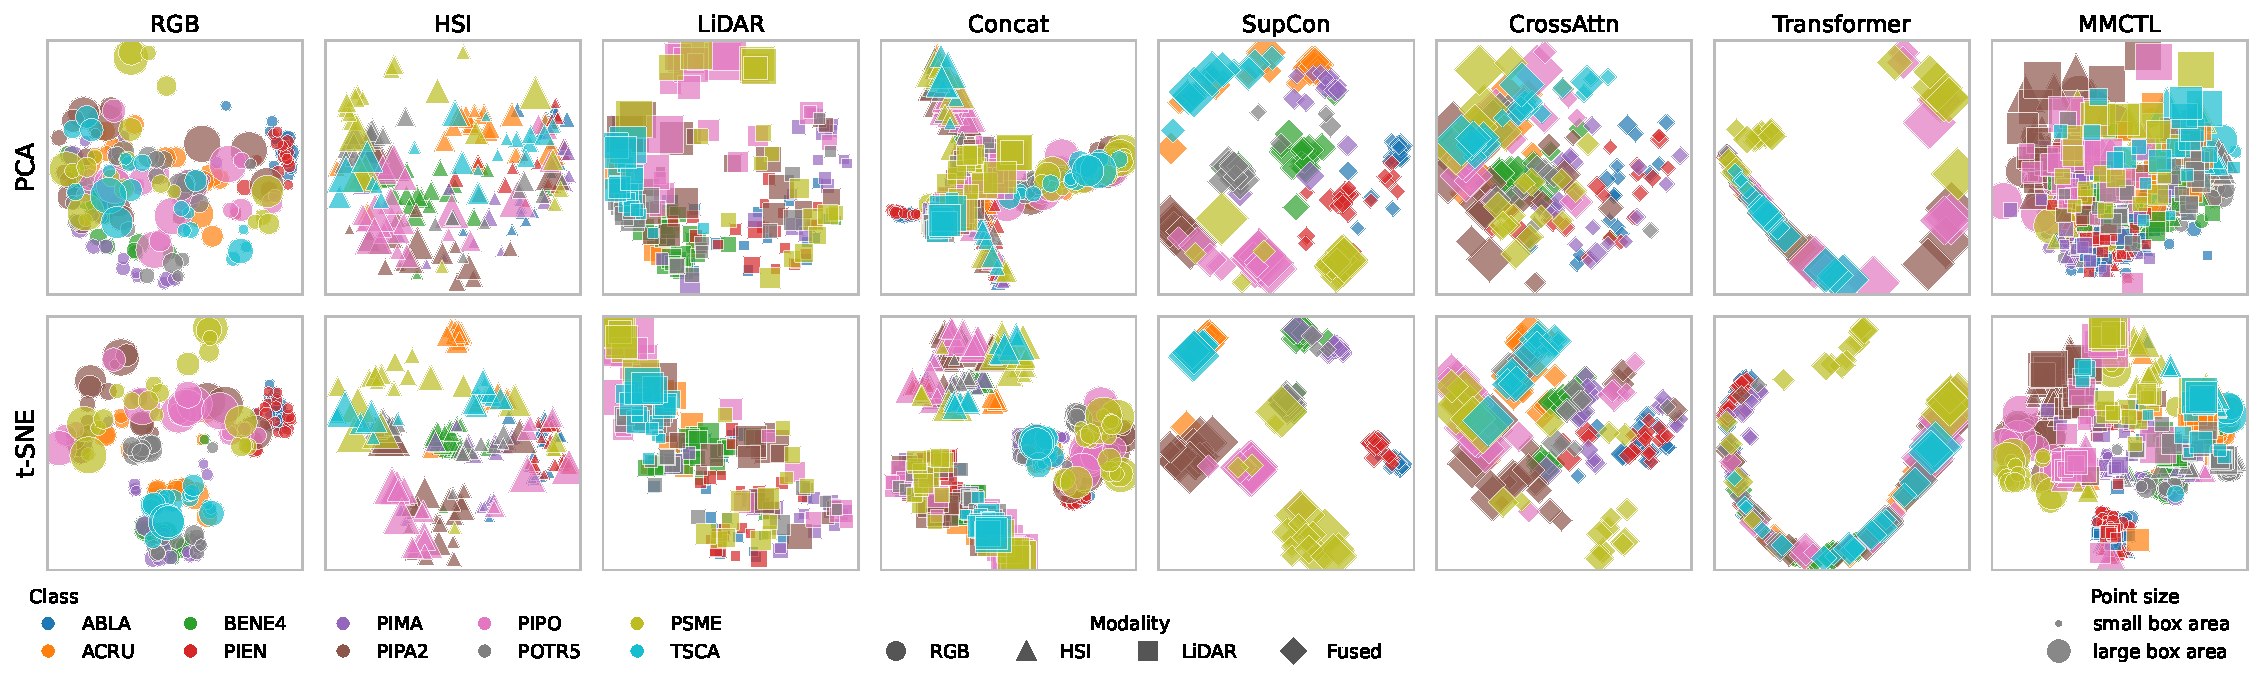
\includegraphics[width=\textwidth]{figures/neon_embedding_space_boxsize.pdf}\\[2pt]
    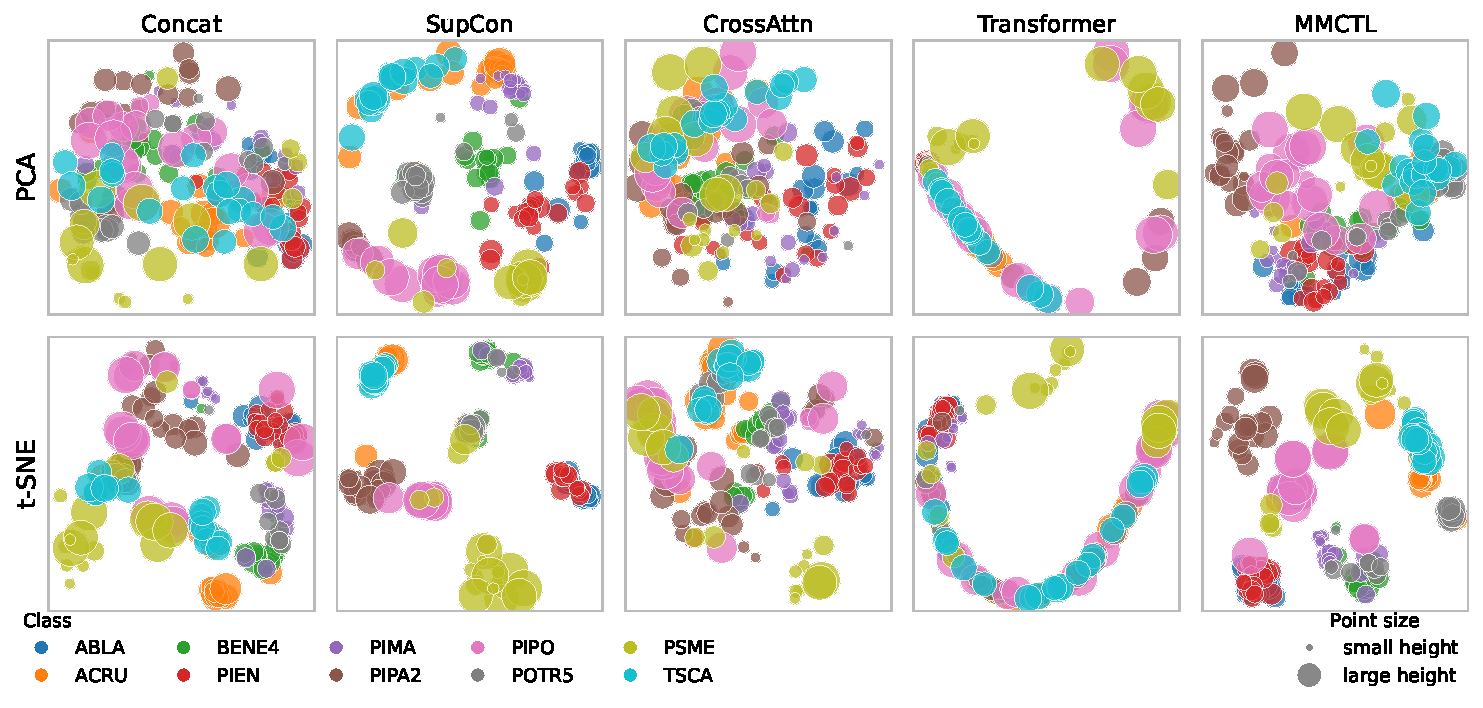
\includegraphics[width=\textwidth]{figures/neon_embedding_space_height.pdf}
    \caption{NEON embedding space across fusion methods (PCA top, t-SNE bottom within each panel row), colored by species. Points are sized by bounding-box area (top block) and by canopy height (bottom block). MMCTL produces species-separated clusters whose point sizes vary smoothly, reflecting continuous box and height geometry, while baselines mix species and lack an ordered geometric gradient.}
    \label{fig:emb_neon}
\end{figure*}

\begin{table}[t]
\centering
\caption{
Downstream task performance using unimodal and fused embeddings. Higher values indicate better performance. Annotation types include C for class labels, B for box, P for position, and H for height annotations.
}
\label{tab:downstream_performance_tasks}
\begin{tabular}{l c c c c}
\toprule
\textbf{Dataset} & \textbf{Method}
& \textbf{C (\%)} $\uparrow$
& \textbf{B $R^2$} $\uparrow$
& \textbf{P $R^2$} $\uparrow$ \\
\midrule
\multirow{7}{*}{AWIR}
& RGB        
& $79.48 \err{1.50}$ 
& $0.41 \err{0.05}$ 
& $0.23 \err{0.08}$ \\
& Thermal    
& $76.98\err{3.14}$ 
& $0.29\err{0.03}$ 
& $0.01 \err{0.04}$ \\
\cmidrule(lr){2-5}
& Concat.    
& $85.21 \err{2.16}$ 
& $0.45\err{0.02}$ 
& $0.27 \err{0.02}$ \\
& SupCon  
& $89.06 \err{1.47}$ 
& $-0.15\err{0.25}$ 
& $-0.37 \err{0.18}$ \\
& CrossAttn    
& $86.67 \err{1.38}$ 
& $0.31\err{0.06}$ 
& $0.06 \err{0.08}$ \\
& Transformer    
& $86.25 \err{1.50}$ 
& $0.04\err{0.12}$ 
& $-0.16 \err{0.13}$ \\
\cmidrule(lr){2-5}
& MMCTL      
& $\mathbf{91.46}\err{1.49}$ 
& $\mathbf{0.62}\err{0.02}$ 
& $\mathbf{0.50}\err{0.05}$ \\
\midrule
\multicolumn{2}{l}{}
& \textbf{C (\%)} $\uparrow$
& \textbf{B $R^2$} $\uparrow$
& \textbf{H $R^2$} $\uparrow$ \\
\midrule
\multirow{8}{*}{NEON}
& RGB        
& $76.22\err{2.33}$ 
& $0.07 \err{0.09}$ 
& $0.32 \err{0.03}$ \\
& HSI        
& $76.22 \err{1.38}$ 
& $0.13 \err{0.06}$ 
& $0.40\err{0.03}$ \\
& LiDAR      
& $48.38 \err{2.09}$ 
& $0.15 \err{0.08}$ 
& $0.67 \err{0.02}$ \\
\cmidrule(lr){2-5}
& Concat.    
& $80.81 \err{1.96}$ 
& $\mathbf{0.36} \err{0.08}$ 
& $\mathbf{0.71} \err{0.01}$ \\
& SupCon  
& $\mathbf{81.42} \err{1.97}$ 
& $0.07 \err{0.14}$ 
& $0.47 \err{0.06}$ \\
& CrossAttn    
& $68.85 \err{2.17}$ 
& $0.27\err{0.10}$ 
& $0.60 \err{0.03}$ \\
& Transformer    
& $43.11 \err{4.50}$ 
& $0.24\err{0.13}$ 
& $0.29 \err{0.06}$ \\
\cmidrule(lr){2-5}  
& MMCTL      
& $80.34 \err{1.03}$ 
& $0.33 \err{0.05}$ 
& $0.63 \err{0.03}$ \\
\bottomrule
\end{tabular}
\end{table}


\subsection{Annotation Weighting and Frozen vs.\ End-to-End Encoders}
\label{subsec:weight-e2e}

\noindent\textbf{Class-weight sensitivity (NEON).}
The joint annotation vector exposes one free knob per task, the weight $w_t$ (Eq.~\eqref{eq:ann-weight}). We sweep the class weight $w_{\text{class}}\in\{0.5,0.8,1.0,1.5\}$ on NEON with the continuous-task weights fixed at $1.0$, using the released full-set MMCTL embeddings under the frozen task-head protocol. As shown in Fig.~\ref{fig:neon_ablation} and Table~\ref{tab:neon_weight_ablation}, increasing $w_{\text{class}}$ sharpens species separation in the embedding space and improves classification accuracy, with a mild trade-off against continuous-attribute regression. This confirms that the weight behaves as intended---trading semantic compactness against geometric spread---and motivates the balanced default used in the main tables.

\begin{figure*}[!htb]
    \centering
    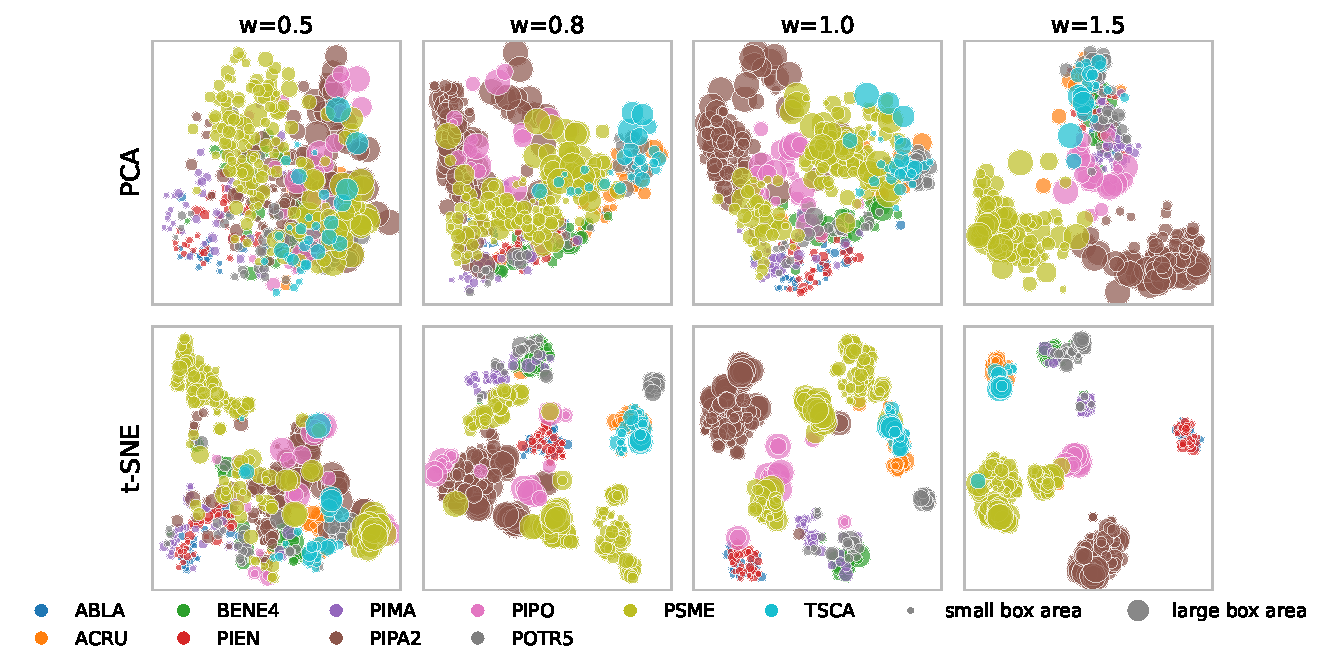
\includegraphics[width=\textwidth]{figures/neon_ablation_classweight_boxsize.pdf}
    \caption{NEON class-weight ablation. MMCTL embeddings trained with class weight $w_{\text{class}}\in\{0.5,0.8,1.0,1.5\}$ (box/height weights fixed at $1.0$), projected with PCA (top) and t-SNE (bottom), colored by species and sized by bounding-box area. Larger class weights yield more compact, better-separated species clusters. (A height-sized version is provided in the supplementary figures.)}
    \label{fig:neon_ablation}
\end{figure*}

%%FILL:neon_weight_ablation_table

\noindent\textbf{Frozen vs.\ end-to-end encoders (NEON).}
The main protocol freezes modality encoders and trains task heads on fixed embeddings. To test whether this frozen choice is justified relative to fine-tuning, we run a controlled comparison on NEON: starting from the same MMCTL-pretrained encoders, we either keep them frozen (main protocol) or unfreeze them and fine-tune end-to-end jointly with the heads, holding the head architecture, data splits, standardized targets, and training budget fixed so the only difference is encoder trainability.
%%FILL:freeze_vs_e2e_result

\subsection{Missing Modality, Compute, and Failure Analysis}
\label{subsec:additional-analyses}

\paragraph{Missing modality.}
As a frozen-embedding probe on released AWIR test embeddings, we zero one $1024$-d half of the $2048$-d MMCTL joint vector (RGB$|$thermal), L2-normalize, and retrain linear probes. Full joint proxy accuracy is $93.44\pm1.37\%$. Dropping thermal yields $84.69\pm2.04\%$ ($-8.75$~pts); dropping RGB yields $86.15\pm1.99\%$ ($-7.29$~pts). Both remain above unimodal RGB/thermal probe accuracies ($\approx$78--80\%), indicating complementary but non-redundant modality use under this probe protocol.

\paragraph{Triplet compute.}
With batch size $32$, modality concatenation yields $64$ embeddings and an upper bound of $249{,}984$ ordered triplets per batch ($\approx 2.0$M per epoch at eight steps) before the annotation-order mask; actual positives are data-dependent. A microbenchmark on Apple M4 CPU measures $\approx 1.7$\,s per training step at batch size $8$; the full AWIR training schedule was not re-timed on this machine.

\paragraph{Cross-modal retrieval.}
Splitting the joint embedding into modality halves and performing cosine nearest-neighbor retrieval gives rank-1 \emph{class} match of $80.8\%$, but rank-1 \emph{identity} match of only $7.5\%$. Failures concentrate on adjacent livestock confusions (e.g., deer$\leftrightarrow$horse, horse$\leftrightarrow$cow; Fig.~\ref{fig:retrieval_failures}). MMCTL therefore preserves class/geometry structure across modalities more reliably than exact instance pairing when joint halves are queried in isolation.

\begin{figure}[!htb]
    \centering
    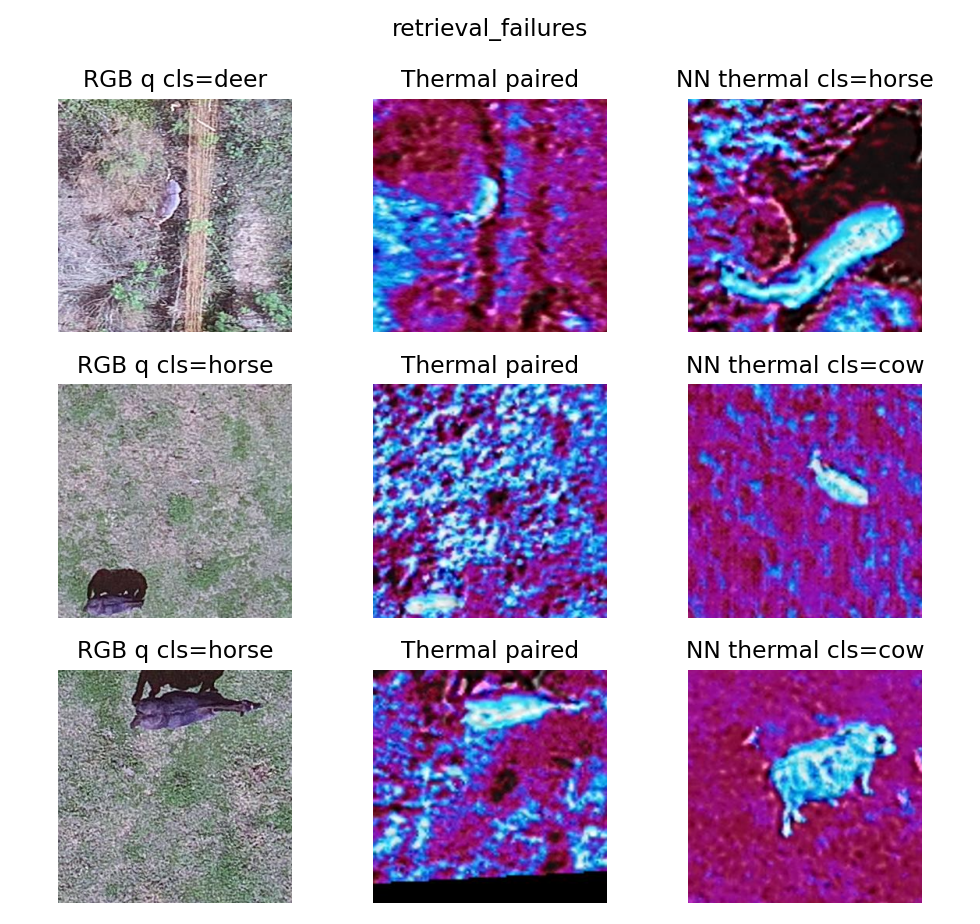
\includegraphics[width=\columnwidth]{figures/awir_retrieval_failures.png}
    \caption{AWIR cross-modal NN failures (RGB half $\rightarrow$ thermal half) for MMCTL joint embeddings. Mismatches are typically adjacent livestock classes rather than arbitrary semantics; identity rank-1 is only $7.5\%$, so we do not claim strong instance retrieval from split halves.}
    \label{fig:retrieval_failures}
\end{figure}

\section{Conclusion}
This work frames multi-modal representation learning as aligning embeddings across sensing modalities using annotation-defined similarity rather than task-loss geometry alone. MMCTL builds a shared latent space by coupling modality-specific embeddings through a weighted joint annotation vector, a margin-free continuous triplet, and pairwise distance alignment, yielding more coherent cross-modal geometry than unimodal or task-driven fusion under the same label sources. AWIR analyses further show statistically significant structure gains, graceful degradation under missing-modality probes, and strong class-level---but not identity-level---cross-modal neighborhoods. Future work includes adaptive annotation weights and end-to-end unfreezing comparisons.



\bibliographystyle{IEEEtran}
\bibliography{paper}




\vfill

\end{document}


